\section{Experimental Results\label{sec:experiment}}
\subsection{Aggregation-based methods perform significantly better than retrieval-based methods (no clustering)}
\begin{figure}[h!]
   \centering
   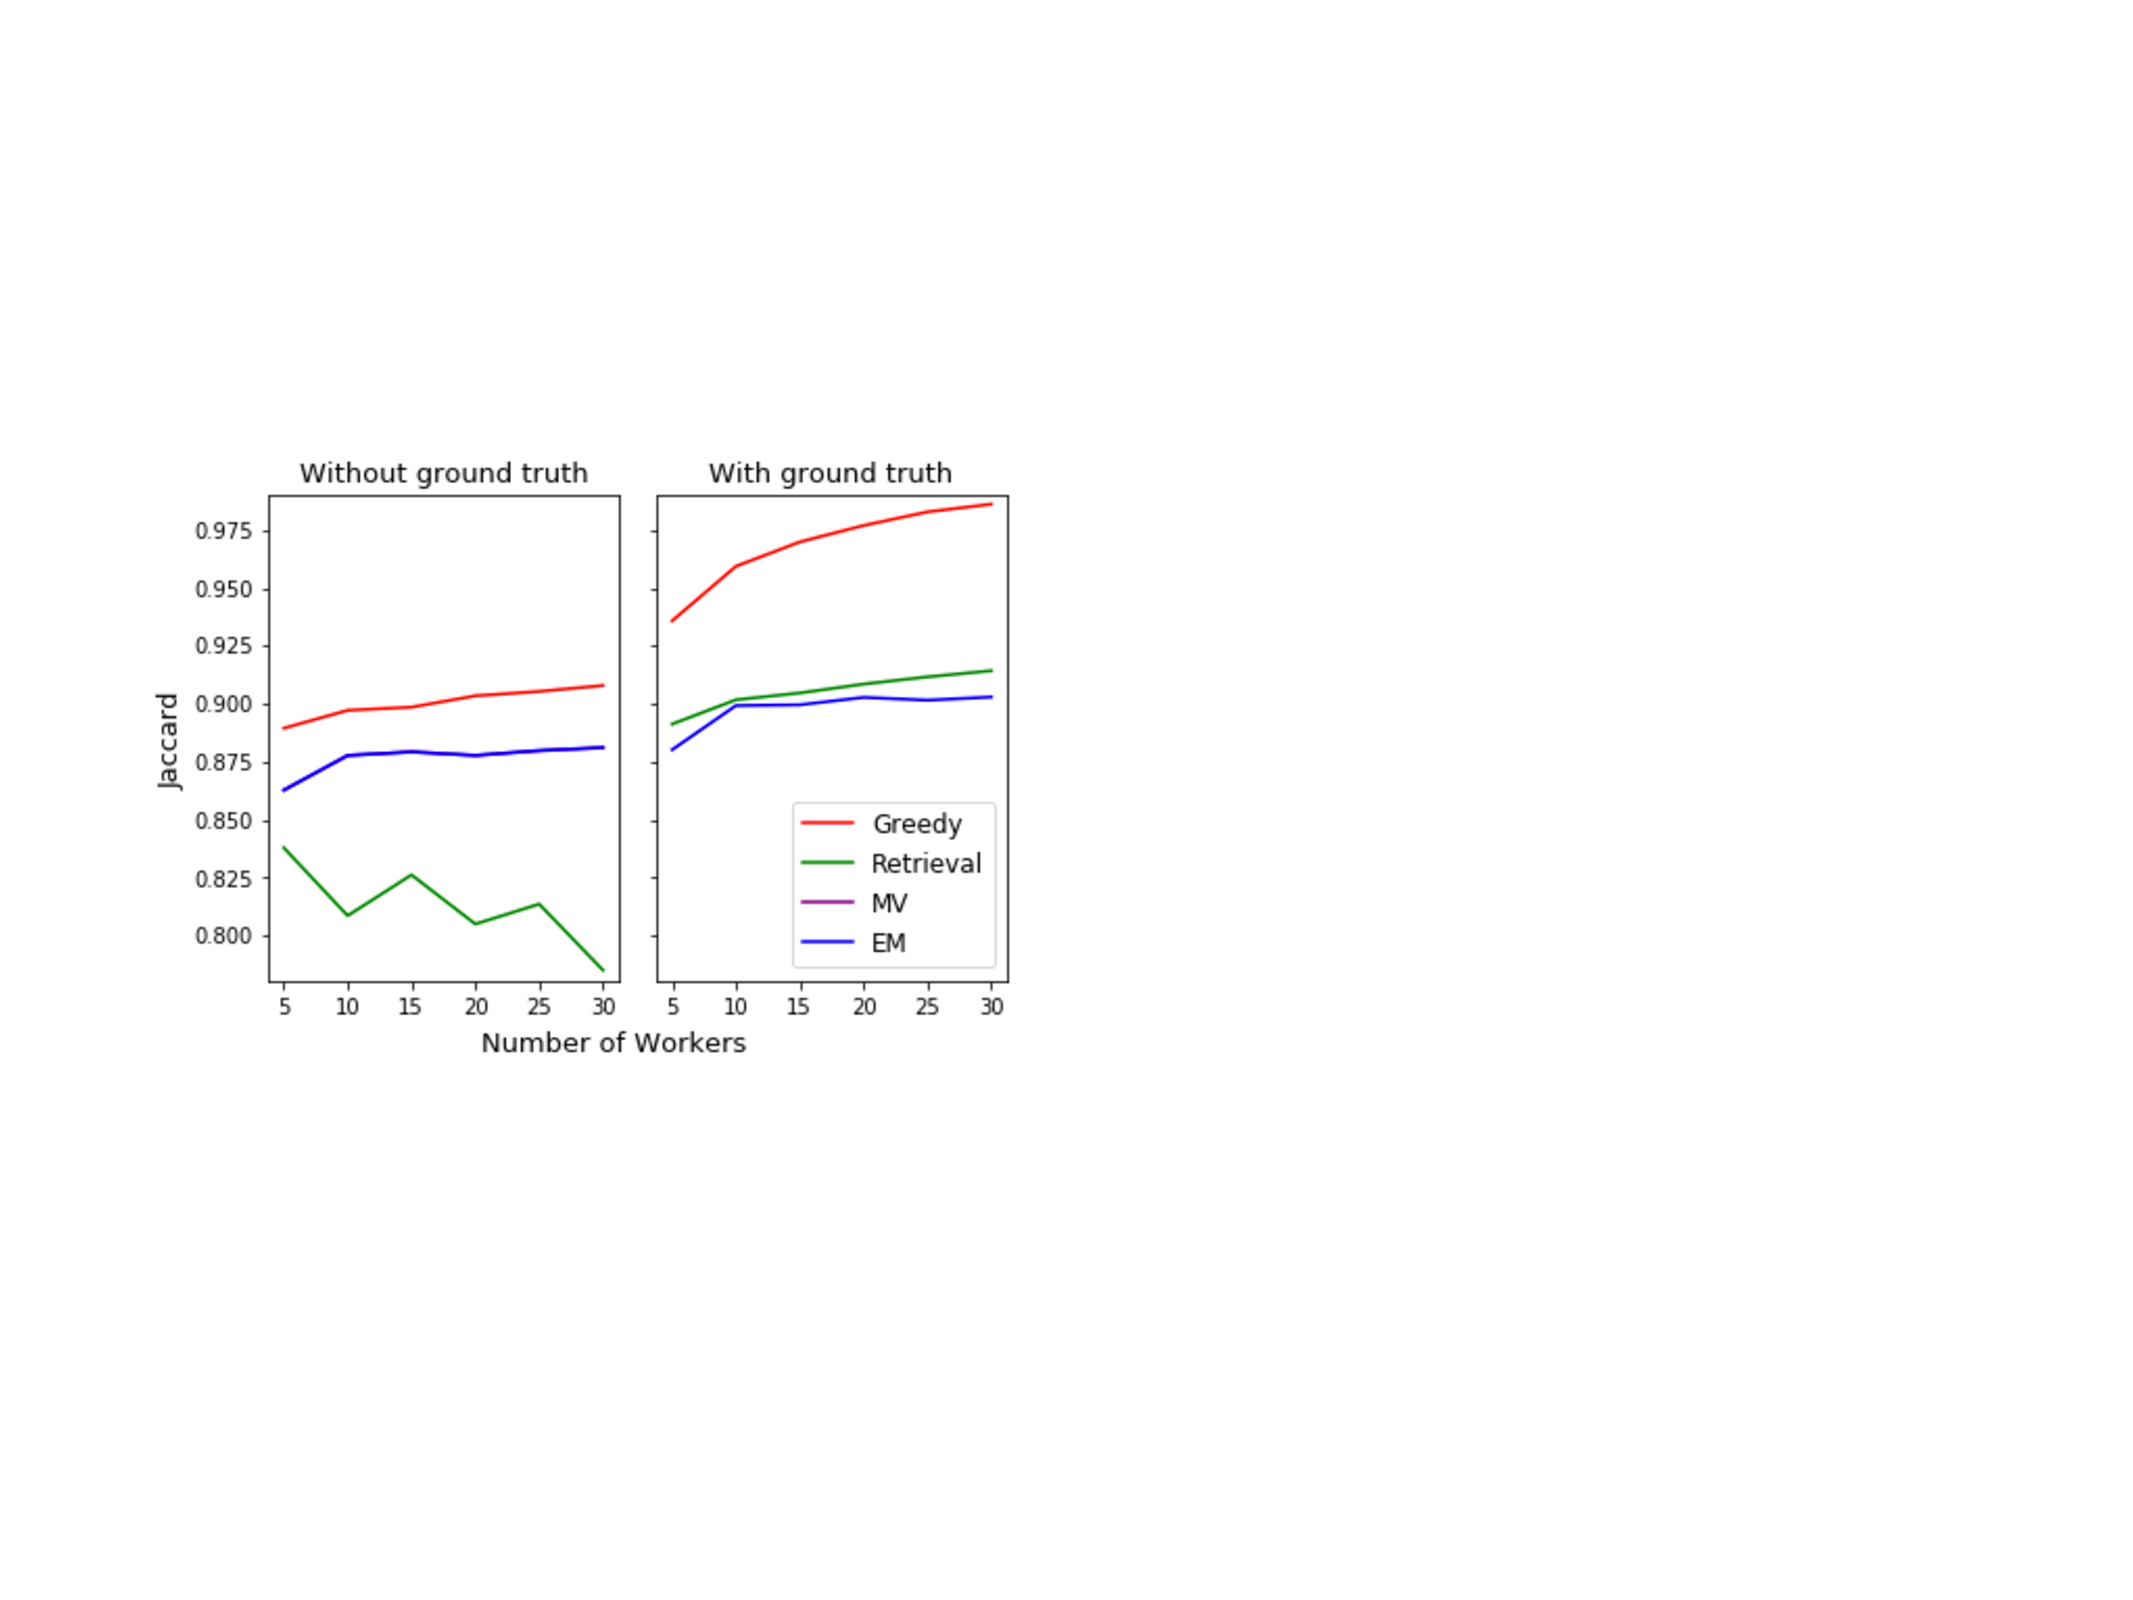
\includegraphics[trim={0 1pt 4pt 0},clip,width=0.8\linewidth]{plots/Retrieval_vs_Aggregation.pdf}
   \caption{Performance of the original algorithms that do not make use of ground truth information (Left) and ones that do (Right). MV and EM results are so close that they overlay on each other.} %\agp{Explain setup for this. How did you generate this?} \dor{not sure what aditya means?}}%Performance comparison between best-performing retrieval and aggregation-based methods. 
   \label{retrieval_vs_aggregation}   
   % \vspace{-12pt}
   % \setlength{\abovecaptionskip}{-30pt}
   % \setlength{\belowcaptionskip}{-23pt}
\end{figure} 
\npar In Figure~\ref{retrieval_vs_aggregation}, we vary the number of worker segmentations along the x-axis and plot the average Jaccard score on the y-axis across different worker samples of a given size across different algorithms. Figure~\ref{retrieval_vs_aggregation} (left) shows that the performance of aggregation-based algorithms (greedy, EM) exceeds the best-achievable through existing retrieval-based method (Retrieval). Then, in Figure \ref{retrieval_vs_aggregation} (right), we estimate the upper-bound performance of each algorithm by assuming that the `full information' based on ground truth was given to the algorithm. For greedy, the algorithm is aware of all the actual tile overlap and non-overlap areas against ground truth, and does not need to approximate these values. For EM, we consider the performance of the algorithm if the true worker quality parameter values (under our worker quality model) are known. For retrieval, the full information version directly picks the worker with the highest Jaccard similarity with respect to the ground truth segmentation. By making use of ground truth information (Figure~\ref{retrieval_vs_aggregation} right), the best aggregation-based algorithm can achieve a close-to-perfect average Jaccard score of 0.98 as an upper bound, far exceeding the results achievable by any single `best' worker (J=0.91). This result demonstrates that aggregation-based methods are able to achieve better performance by performing inference at the tile granularity, which is guaranteed to be finer grained than any individual worker segmentation. 

\subsection{The performance of aggregation-based methods scale well as more worker segmentations are added.}
\par \noindent Intuitively, larger numbers of worker segmentations result in finer granularity tiles for the aggregation-based methods. The first row in Table~\ref{statsTable} lists the average percentage change in Jaccard between 5-workers and 30-workers samples, demonstrating a monotonically increasing relationship between number of worker segmentations used and the performance. However, retrieval-based methods do not benefit from more segmentations.

\subsection{Clustering as preprocessing improves algorithmic performance.}
\par \noindent The average percentage change between the no clustering and clustering results is shown in Table~\ref{statsTable}. Clustering generally results in an accuracy increase. Since the `full information' variants are already free of semantic ambiguity and errors, clustering does not assist with further improvement. %In particular, we see a greater improvement with clustering preprocessing for algorithms that are not very robust in resolving semantic errors or ambiguity, such as for the \texttt{num pts} retrieval algorithm, than compared to the aggregation-based methods. 
\begin{table}[h!]
   \small
     % \setlength\tabcolsep{1.5pt}
      \begin{tabular}{l|l|l|l|l|l|l|l}
      & \multicolumn{3}{c|}{Retrieval-based} & \multicolumn{4}{l|}{Aggregation-based} \\
      Algorithm         & num pts     & worker    & worker*    & MV     & EM     & greedy   & greedy*   \\ \hline
      Worker Scaling    & -6.30       & -0.25     & 2.58       & 1.63   & 1.64   & 2.16     & 5.59      \\ \hline
      Clustering Effect & 5.92        & 4.00      & -0.02      & 2.05   & 1.38   & 5.55     & -0.06    
      \end{tabular}
      \vspace{10pt}
      \caption{Jaccard percentage change due to worker scaling and clustering. Algorithms with * makes use of ground truth information.}
      \label{statsTable}
\end{table}
\par The clustering preprocessing step can significantly improve performance of algorithms that are not very robust to segmentations with semantic errors or ambiguities, such as the heuristic-based number of points approach. When examining the gap of increase with and without clustering in Figure \ref{cluster_effect}, we find that aggregation-based methods performs better than retrieval-methods exhibits a smaller gap between the performances. This effect is due to aggregation-based method's higher performance in the no cluster case, indicating that it is able to capture some of the semantic ambiguities and errors in the dataset.
\begin{figure}[ht!]
      \centering
      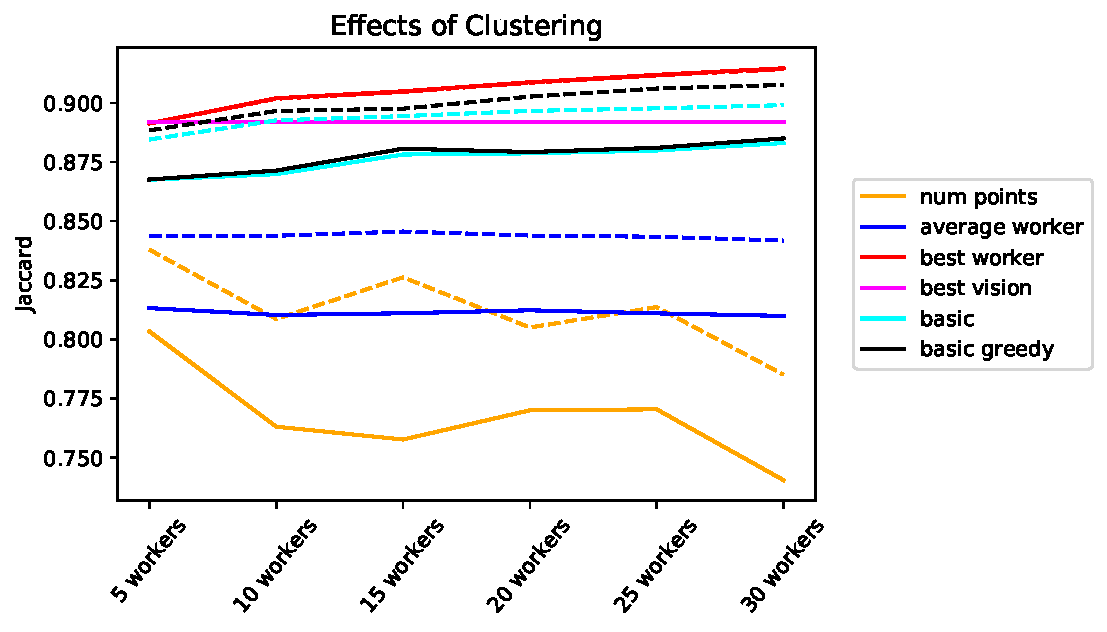
\includegraphics[width=\textwidth]{plots/Effects_of_clustering.pdf}
      \caption{Performance comparisons between averaging over experiments with clustering as a preprocessing step(dotted) and the unclustered cases(solid) for different algorithms.}
      \label{cluster_effect}
\end{figure}


\subsection{Overall: with clustering + our algo > baseline}


\subsection{How well does the inferred worker qualities predict individual worker performance?}
    \subsubsection{Correlation of worker qualities against performance}
     To further investigate how the EM models are performing, we looked at whether the model-inferred worker qualities is indicative of the actual quality of a segmentation. We performed linear fitting independently for each sample-objects and computed the $R^2$ statistics to determine whether worker qualities can accurately predict precision, recall, and Jaccard scores. Visual inspection of the basic worker quality model fitting showed that for objects that suffered from type two errors (semantic ambiguity), the single-parameter worker quality was unable to capture the overbounding behavior, which lead to a low precision and Jaccard. The results are listed in Table \ref{correlation} to highlight how our advanced worker qualities were able to better capture these scenarios. The clustering preprocessing was not performed for the values in Table \ref{correlation} to demonstrate the sole effect of the EM algorithm. Nevertheless, our clustered results also show a similar trend, with an average of $R^2$=0.88 and 0.89 for the GT and GTLSA models across all objects respectively. We also find that in general the linear fit improves as the number of data points increases, which indicates consistency in the fitted model.
    \begin{table}[ht!]
    \small
      \begin{tabular}{ccccccc}
        \hline
           N &   basic &   GT &   GTLSA &   isobasic &   isoGT &   isoGTLSA \\
        \hline
              5 &      0.601 &   0.907 &      0.901 &       0.576 &    0.907 &       0.904 \\
            10 &      0.632 &   0.895 &      0.899 &       0.633 &    0.895 &       0.898 \\
            15 &      0.622 &   0.897 &      0.898 &       0.622 &    0.897 &       0.897 \\
            20 &      0.636 &   0.894 &      0.899 &       0.637 &    0.894 &       0.898 \\
            25 &      0.66  &   0.901 &      0.905 &       0.661 &    0.901 &       0.904 \\
            30 &      0.673 &   0.907 &      \cellcolor{blue!25}0.914 &       0.676 &    0.907 &       \cellcolor{blue!25}0.913 \\
        \hline
      \end{tabular}
        \caption{Linear correlation of worker qualities against ground truth performance for different quality models across different number of workers (N). The lower worker samples exhibit lower $R^2$ due to the variance from smaller number of datapoints for each independent fit. }
        \label{correlation}
    \end{table}
    \vspace{-10pt}
    % \subsubsection{EM performance with different worker quality models}
    %   - why is iso cases not performing as well
    \subsubsection{Best worker quality retrieval}
    One application of worker qualities is that it could be used as an annotation scoring function for retrieving the best quality worker segmentation. We explore this approach by training a linear regression model for every sample-object and use the worker qualities to predict the precision, recall, and Jaccard of individual worker annotations against ground truth. Then, we query the model with the inferred worker quality and retrieve the worker with the best predicted Jaccard. 
    \par The reason why a linear regression model was chosen rather than simply sorting the worker qualities and picking the best is that sorting based on multiple worker qualities (precision, recall, Jaccard) effectively applies equal weighting to all quality attributes, whereas our advanced models are specifically designed to capture cases of false-positives and false-negatives that can yield drastically different recall and precision values. We have tested that the linear regression model performs better on this task that simple sorting is capable of learning the weights that helps it make better predictions. As shown in Table~\ref{bigtable}, the performance of worker-quality based retrieval is comparable the performance other aggregation-based methods. We find that amongst the different worker quality models, advanced worker quality models perform the best, agreeing with our intuition regarding correlation results observed in Table~\ref{correlation}.
    \begin{table}[ht!]
    \small
    \setlength\tabcolsep{3pt}
    \begin{tabular}{lrrrrrr}
      \hline
       algo/N                  &     5 &    10 &    15 &    20 &    25 &    30 \\
      \hline
       num points           & 0.838 & 0.809 & 0.826 & 0.805 & 0.814 & 0.785 \\
       best worker          & 0.891 & 0.902 & 0.905 & 0.909 & 0.912 & 0.914 \\
       \hline
       MV                   & 0.885 & 0.893 & 0.894 & 0.897 & 0.898 & 0.899 \\
       EM[basic]           & 0.884 & 0.893 & 0.894 & 0.897 & 0.898 & 0.899 \\
       EM[GT]              & 0.885 & 0.893 & 0.894 & 0.897 & 0.898 & 0.899 \\
       EM[GTLSA]           & 0.871 & 0.892 & 0.891 & 0.896 & 0.897 & \cellcolor{blue!25} 0.899 \\
       greedy               & 0.888 & 0.896 & 0.896 & 0.902 & 0.905 & 0.906 \\
       wqr[basic]          & 0.878 & 0.877 & 0.877 & 0.877 & 0.878 & 0.878 \\
       wqr[GT]             & 0.884 & 0.885 & 0.885 & 0.885 & 0.887 & 0.887 \\
       wqr[GTLSA]          & 0.874 & 0.881 & 0.883 & 0.885 & 0.886 & \cellcolor{blue!25} 0.887 \\
      \hline
    \end{tabular}
    \caption{Summary of average performance across workers with clustering applied as preprocessing in all algorithms across different number of workers (N). wqr is the abbreviation for best worker quality retrieval methods.}
    \label{bigtable}
    \end{table}